\chapter{Analysis and Results}
\section{Linearity of the TEPX luminometers}
The linearity of the detector is an important parameter. The determination of the calibration constants is done by performing a vdM scan, however, vdm scans are performed at considerably low pileup, $\mu=0.5$, and it is then extrapolated to a pileup of $\approx 200$, this extrapolation generates a significant source of uncertainty. An ideal detector will demonstrate a linear relation between the measured event rate, and the instantaneous luminosity. This also implies a linear relation between the event rate and the pileup:
\begin{equation}
    \left\langle N_{\text {clusters/int}}\right\rangle=\frac{\left\langle N_{\text {cluster}}\right\rangle}{\mu}=\frac{\sigma_{\text {vis}}}{\sigma_{\text {tot}}}
\end{equation}
\begin{equation}
     \left\langle N_{\text {clusters}}\right\rangle=\frac{\sigma_{\text {vis}}}{\sigma_{\text {tot}}}\mu
\end{equation}

Different sources can affect the linearity of a detector, such as, efficiency factors depending on single bunch instantaneous luminosity, short-term effects, like overall rate-dependent efficiency factors, out-of-time effects due to late arriving particles, etc. At CMS, the monitoring and corrections to linearity are performed using emittance scans \cite{CMS-PAS-LUM-18-002}. Emittance scans are used to correct the measured event rate in each fill, for efficiency and linearity.

As mentioned before, the TEPX luminometers use two different observables when measuring the event rate, pixel clusters and two-fold coincidences. A linear response from the TEPX and TEPXD4R1 luminometers is a must, for a precise luminosity measurement. To see the response of the luminometers, the number of clusters/coincidences per event is histogrammed, using data form the hige pileup simulation, this is done for each ring and disk of the luminometer. In the case of coincidences in r, the histograms are created per set of rings. Once the distribution for each histogram is obtained, the mean of these distributions is plotted as a function of pileup. A line is fitted to the lowest pileup values, from 0 to 2, to simulate vdm scan conditions. This line is then extrapolated up to a pileup of 200. Figures \ref{lin1}-\ref{lin4} show these fits, where the deviations from the straight line are found to be less than $1\%$. The linearity of the detector was the main source of uncertainty during Run 2, how ever, this is not the only one, other sources include afterglow, x-y nonfactorization, cross-detector consistency, etc, but these types of uncertainties can only be estimated during regular physics runs \cite{CMS-PAS-LUM-18-002}.


\begin{center}
    \begin{figure}[H]
\begin{minipage}[b]{0.5\linewidth}
        \centering
        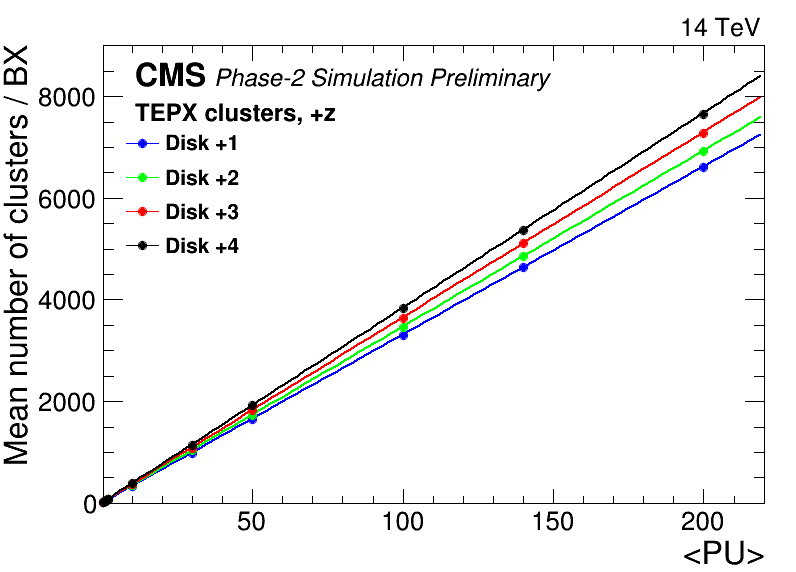
\includegraphics[scale=0.25]{Chapter4/plots/TEPX_totalcluster_linearity.png}
\end{minipage}
\begin{minipage}[b]{0.5\linewidth}
        \centering
        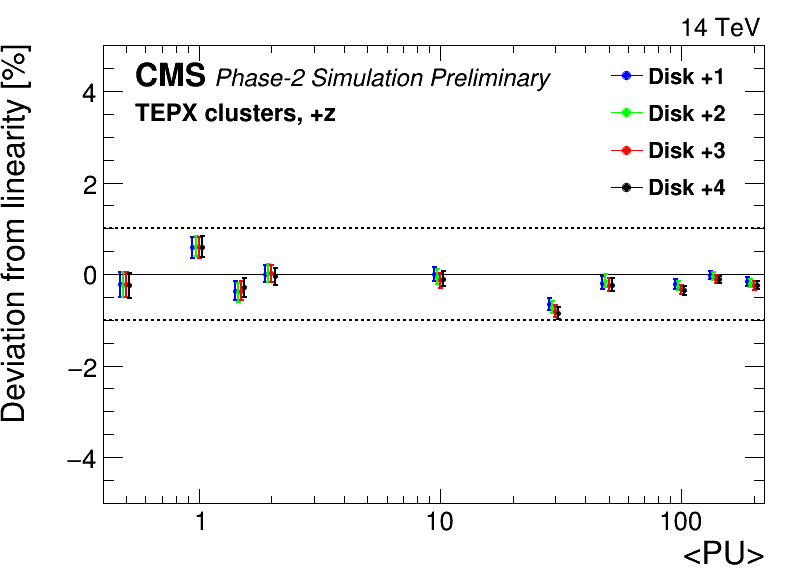
\includegraphics[scale=0.25]{Chapter4/plots/TEPX_totalcluster_residuals.png}
\end{minipage}
    \caption[Linearity of TEPX for pixel clusters.]{\textit{Left}: Simulated mean number of pixel cluster per bx for the each disk of TEPX, as a function of pileup. A line is fitted between the pileup values of 0 and 2, and the extrapolated to higher pileup values. \textit{Right}: Deviation from linearity for clusters for TEPX. The nonlinearity is calculated as the relative difference between the points and the fitted function.  }
    \label{lin1}
\end{figure}
\end{center}
\begin{center}
    \begin{figure}[H]
\begin{minipage}[b]{0.5\linewidth}
        \centering
        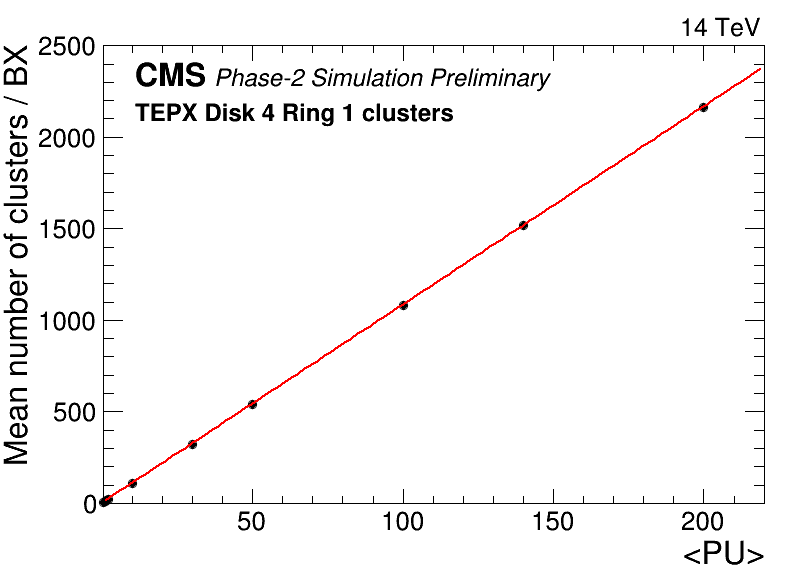
\includegraphics[scale=0.25]{Chapter4/plots/TEPX_Disk_4_Ring_1_mean_number_of_clusters___bx_Linearity.png}
\end{minipage}
\begin{minipage}[b]{0.5\linewidth}
        \centering
        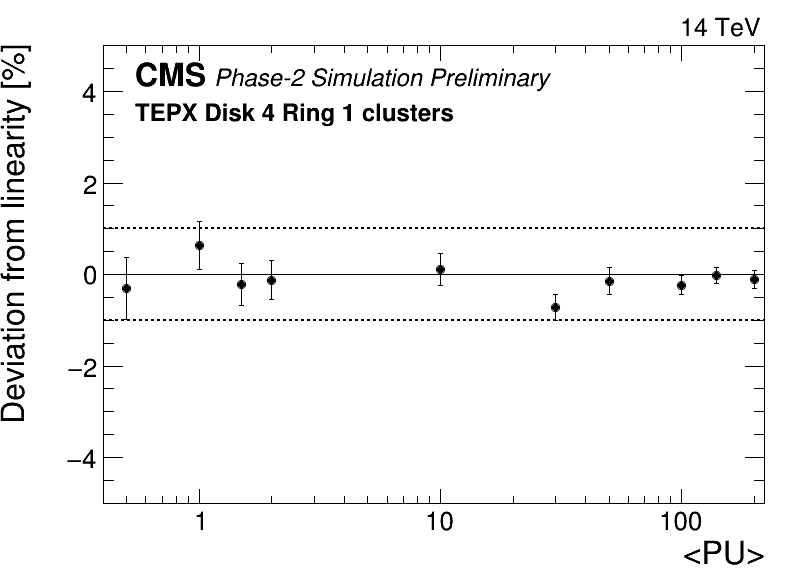
\includegraphics[scale=0.25]{Chapter4/plots/TEPX_Disk_4_Ring_1_mean_number_of_clusters___bx_Linearity_residuals.png}
\end{minipage}
    \caption[Linearity of TEPXD4R1 for pixel clusters.]{\textit{Left}: Simulated mean number of pixel cluster per bx for the entirety of TEPXD4R1, as a function of pileup. A line is fitted between the pileup values of 0 and 2, and the extrapolated to higher pileup values. \textit{Right}: Deviation from linearity for clusters for TEPXD4R1. The nonlinearity is calculated as the relative difference between the points and the fitted function.}
    \label{lin2}
\end{figure}
\end{center}


\begin{center}
    \begin{figure}[H]
\begin{minipage}[b]{0.5\linewidth}
        \centering
        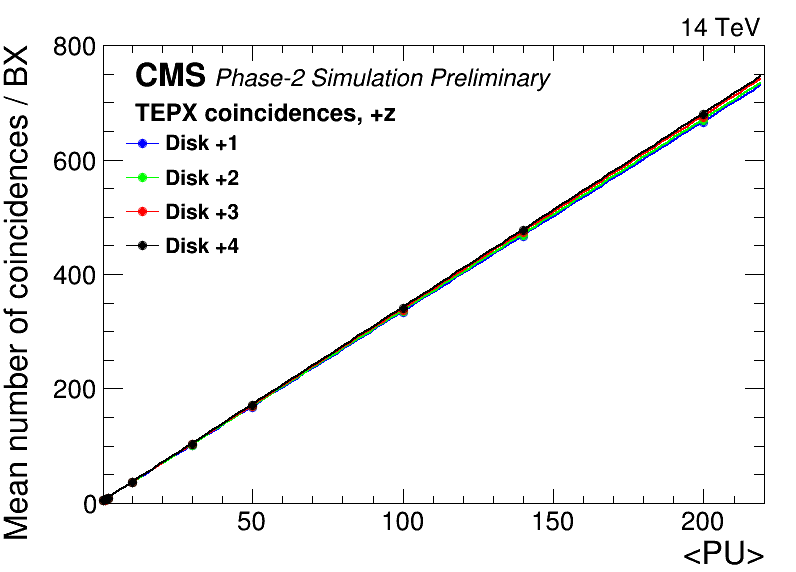
\includegraphics[scale=0.25]{Chapter4/plots/TEPX_coincidences_Linearity.png}
\end{minipage}
\begin{minipage}[b]{0.5\linewidth}
        \centering
        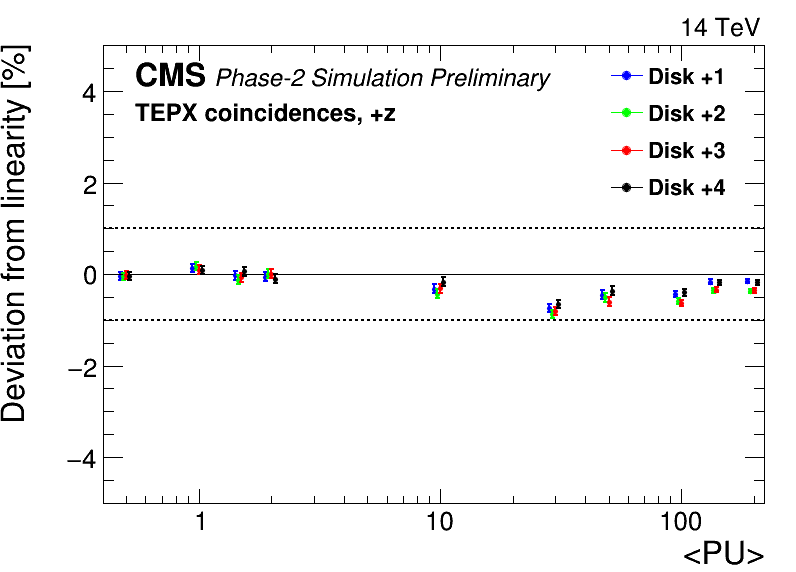
\includegraphics[scale=0.25]{Chapter4/plots/TEPX_coincidences_Linearity_residuals.png}
\end{minipage}
    \caption[Linearity of TEPX for two-fold coincidences.]{\textit{Left}: Simulated mean number of two-fold coincidences per bx for the each disk of TEPX, as a function of pileup. A line is fitted between the pileup values of 0 and 2, and the extrapolated to higher pileup values. \textit{Right}: Deviation from linearity for clusters for TEPX. The nonlinearity is calculated as the relative difference between the points and the fitted function.}
    \label{lin3}
\end{figure}
\end{center}
\begin{center}
    \begin{figure}[H]
\begin{minipage}[b]{0.5\linewidth}
        \centering
        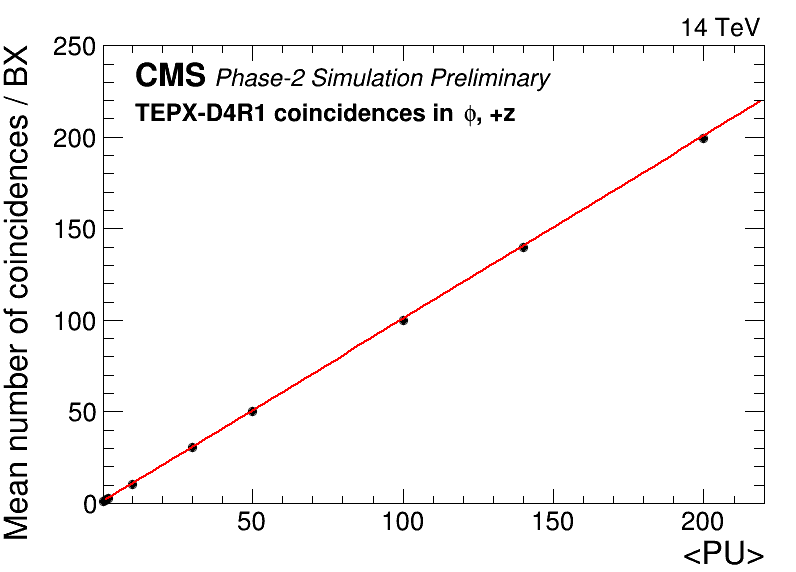
\includegraphics[scale=0.25]{Chapter4/plots/TEPX_Disk_4_Ring_1_mean_number_of_coincidences___bx_Linearity.png}
\end{minipage}
\begin{minipage}[b]{0.5\linewidth}
        \centering
        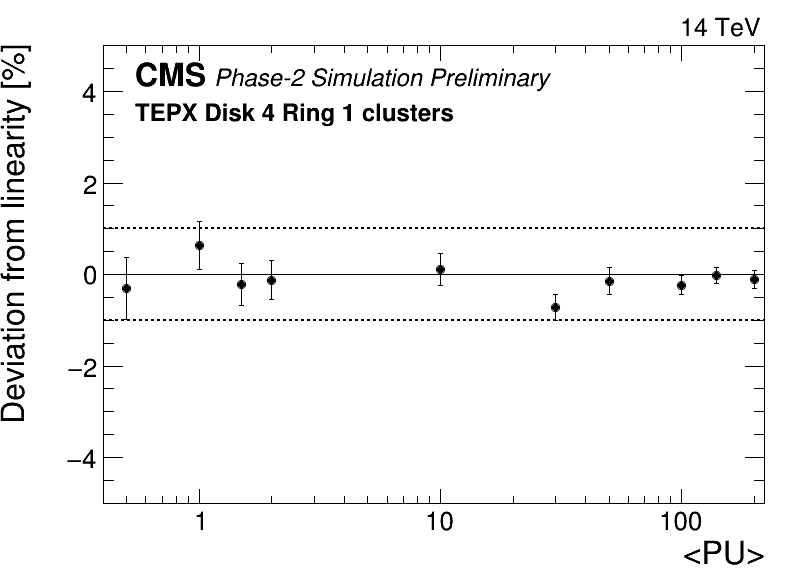
\includegraphics[scale=0.25]{Chapter4/plots/TEPX_Disk_4_Ring_1_mean_number_of_clusters___bx_Linearity_residuals.png}
\end{minipage}
    \caption[Linearity of TEPXD4R1 for two-fold coincidences.]{\textit{Left}: Simulated mean number of two-fold coincidences per bx for the entirety of TEPXD4R1, as a function of pileup. A line is fitted between the pileup values of 0 and 2, and the extrapolated to higher pileup values. \textit{Right}: Deviation from linearity for clusters for TEPXD4R1. The nonlinearity is calculated as the relative difference between the points and the fitted function.}
    \label{lin4}
\end{figure}
\end{center}
\pagebreak



%%%%%%%%%%%%%%%%%%%%%%%%%%%%%%%%%%%%%%%%%%%%%%%%%%%%%%%%%%%%%%%%%%%%%%%%%%%%%%%%%%
\section{Statistical precision for Physics data taking}
The statistical precision of the luminometers is a very important parameter, the precision at which the event rate is determined is another statistical uncertainty considered when calculating the luminosity. The goal for the HL-LHC is to achieve an accuracy of $1\%$ for luminosity measurements, for this, a subpercentage precision is desired for all luminometers. The instantaneous luminosity  expected for the HL-LHC is of $7.5\times10^{34}$ $cm^{-2}s^{-1}$, almost 4 times the luminosity reached during Run 2 of the LHC. This value of luminosity can only be achieved if the number of proton-proton interactions per bunch (pileup), is equal or close to 200, during regular physics runs. 

The statistical precision of the TEPX and TEPXD4R1 luminometers was calculated using:
\begin{equation}
\text {Relative statistical precision} \%=100\times \frac{\sqrt{N}}{N}
\label{statpr}
\end{equation} 
where $N$ is the mean number of pixel clusters/coincidences per event measured by the detector, for a given integration period, and is given by 
\begin{equation}
N=(\text {Number of counts per event})\times(\text {Trigger Frequency per bx})\times(\text {Time integration period})
\label{N01}
\end{equation}
 the Trigger Frequency per bx is 
\begin{equation}
\text {Trigger Frequency per bx}= \frac{\text {Total Readout Frequency}}{\text {Total Number of bx (3564)}}
\label{tfb}
\end{equation}
Assuming total readout frequency is uniformly distributed across all bunch crossings.

During regular physics runs, the TEPXD4R1 luminometer will run at a Total Readout Frequency of 825kHz, while the TEPX luminometer will run at 75kHz. The Number of counts per event is taken from simulated measurements using Run 2 data, specifically from the 2018 data taking period. The statistical precision of  the TEPX luminometers, for pixel clusters and two-fold coincidences (2x coincidences), is shown in Table \ref{tepxstat}.
\begin{table}[H]
\centering
\caption[Statistical precision of the TEPX luminometers in \% for pileup 200.]{Statistical precision of the TEPX luminometers in \% for pileup 200. Columns shown are the luminometer readout frequency, and estimated precision for 1 bunch crossing and 2748 colliding bunches for integrated of 1s.}
\scalebox{.8}{
\begin{tabular}{|l | c | c | c |}
\hline
 & Readout Frequency (kHz)& 1 bx, 1s &2748 bx, 1s   \\
\hline
TEPXD4R1 Clusters&825&0.1&0.0019\\
\hline
TEPXD4R1 2x Coincidences&825&0.31&0.006\\
\hline
TEPX Clusters&75&0.095&0.0018\\
\hline
TEPX 2x Coincidences&75&0.34&0.0066\\
\hline
\end{tabular}}
\label{tepxstat}
\end{table}

%%%%%%%%%%%%%%%%%%%%%%%%%%%%%%%%%%%%%%%%%%%%%%%%%%%%%%%%%%%%%%%%%%%%%%%%%%%%%%%%%


%%%%%%%%%%%%%%%%%%%%%%%%%%%%%%%%%%%%%%%%%%%%%%%%%%%%%%%%%%%%%%%%%%%%%%%%%%%%%%%%%%%%%%%%%%%%
\section{Statistical precision for vdM }
The vdM scan is performed under special conditions, in order to determine the calibration constant $\sigma_{vis}$ as accurately as possible. The scan is performed at a low pileup of 0.5, this is done since the specific precision needed to determine $\sigma_{vis}$ cannot be reached during regular physics runs with higher pileup. Once  $\sigma_{vis}$ is determined, it can be used during regular physics runs, this is because the detector's acceptance should not change under either of the two conditions. 

The scan's duration is of 30 seconds per step, in which event rate measurements are taken. The precision at which these measurements are taken, will determine the precision with which the calibration constant is determined, among other things. The statistical precision for event rates during a vdM scan is calculated with equation \ref{statpr}, using the same data used for physics runs. To simulate the lower pileup, the mean number of clusters/coincidences per event is divided by 400, since that data corresponds to a pileup of 200.  During vdM scans the TEPX and TEPXD4R1 will run at a higher trigger frequency of 1MHz and 2 MHz respectively. This is to make up for the low event rates due to the low amount of interaction.  Table \ref{vdmpre} shows the statistical precision for different numbers of bunches as well as different integration periods.

\begin{table}[ht]
\centering
\caption[Statistical precision of the TEPX luminometers in \% for pileup 0.5.]{Statistical precision of the TEPX luminometers in \% for pileup 0.5. Columns shown are the luminometer readout frequency, estimated precision for 1bx per 1 s integration, and 1 and 150 bx for 30 s integration period.}
\scalebox{.8}{
\begin{tabular}{|l | c | c | c |c|}
\hline
  & Readout Frequency (kHz) &1 bx, 1s & 1 bx, 30s & 150 bx, 30s\\
\hline
TEPXD4R1 Clusters&2000&1.3&0.23 & 0.019\\
\hline
TEPXD4R1 2x Coincidences&2000&4.07&0.74 & 0.060\\
\hline
TEPX Clusters&1000&0.52&0.095 & 0.0077\\
\hline
TEPX 2x Coincidences&1000&1.9&0.34 & 0.028\\
\hline
\end{tabular}}
\label{vdmpre}
\end{table}
%%%%%%%%%%%%%%%%%%%%%%%%%%%%%%%%%%%%%%%%%%%%%%%%%%%%%%%%%%%%%%%%%%%%%%%%%%
\subsection{Toy simulation of the vdM scan}
Using the results from the previous section a vdm scan toy study was created to calculate the statistical uncertainty for $\sigma_{vis}$. To simulate the event rate measurements, a Gaussian distribution is used:
\begin{equation}
    R(\Delta x)= N_0 e^{\frac{(\Delta x-x_0)}{2\Sigma_x^2}}
    \label{toyvdm}
\end{equation}
where $ R(\Delta x)$ is the measured event rate, $\Delta x$ is the beam separation in the x axis, $N_0$ is the mean number of cluster/coincidences per event for 1 bx in a 30 s integration period and $\Sigma_x$ is the beam overlap width. The toy study simulates 25 steps for the vdM scan, that is, 25 event rate measurements, and uses a beam overlap width of $\Sigma_x=120$ mm. The statistical uncertainty for each measurement was calculated using
\begin{equation}
    \text { statistical uncertainty}=\sqrt{R(\Delta x)}
    \label{uncvdm}
\end{equation}
Once the measurements have been histogramed as a function of beam separation $\Delta x$, another Gaussian distribution is fitted to the measurements to simulate vdM scan process for determining $\sigma_{vis}$. Figures \ref{ref1} and \ref{ref2} show the results of this process for TEPX and TEPXD4R1 luminometers for pixel cluster and coincidences.
\begin{center}
    \begin{figure}[H]
\begin{minipage}[b]{0.5\linewidth}
        \centering
        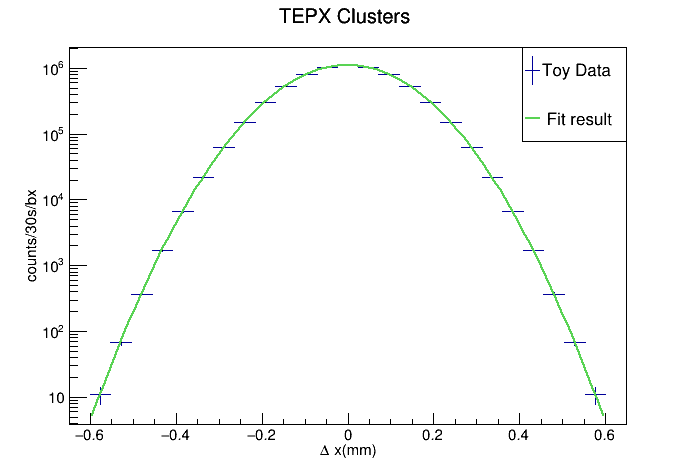
\includegraphics[scale=0.3]{Chapter4/plots/toy_cTEPX.png}
\end{minipage}
\begin{minipage}[b]{0.5\linewidth}
        \centering
        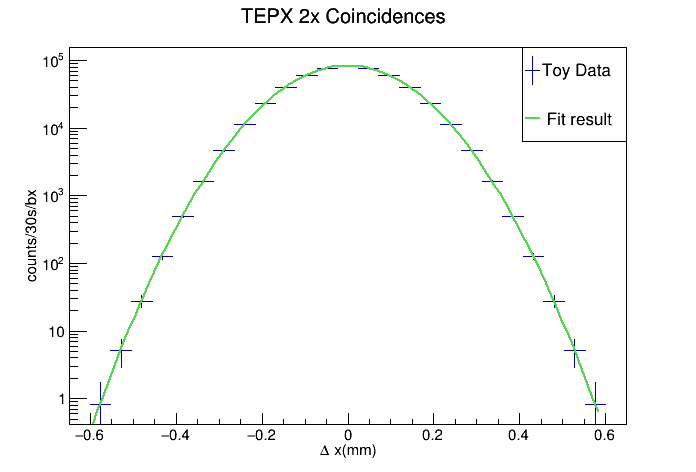
\includegraphics[scale=0.3]{Chapter4/plots/toy_2xTEPX.png}
\end{minipage}
    \caption[Simulated rate measurements of the vdM toy study for TEPX.]{Simulated rate measurements for pixel clusters (Left), coincidences (Right), and their corresponding uncertainties (blue lines) for TEPX, during a vdM scan. The green line corresponds to the fitted Gaussian distribution.}
    \label{ref1}
\end{figure}
\end{center}
\begin{center}
    \begin{figure}[H]
\begin{minipage}[b]{0.5\linewidth}
        \centering
        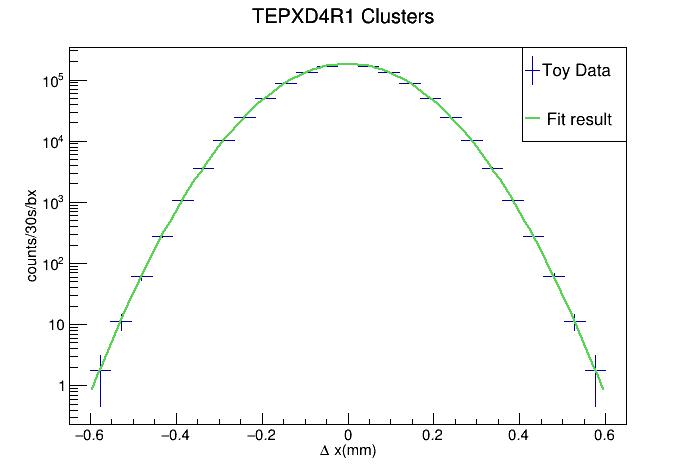
\includegraphics[scale=0.3]{Chapter4/plots/toy_cD4R1.png}
\end{minipage}
\begin{minipage}[b]{0.5\linewidth}
        \centering
        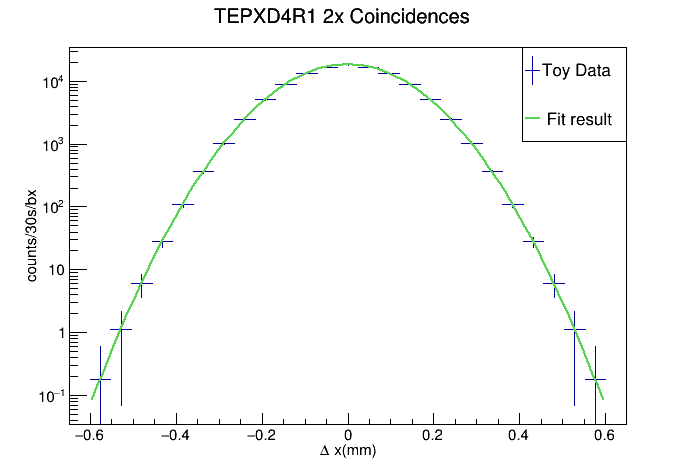
\includegraphics[scale=0.3]{Chapter4/plots/toy_2xD4R1.png}
\end{minipage}
    \caption[Simulated rate measurements of the vdM toy study for TEPXD4R1.]{Simulated rate measurements for pixel clusters (Left), coincidences (Right), and their corresponding uncertainties (blue lines) for TEPXD4R1, during a vdM scan. The green line corresponds to the fitted Gaussian distribution.}
    \label{ref2}
\end{figure}
\end{center}


Once the histograms is fitted with a Gaussian distribution, the mean number of counts per event $N_0$, the beam overlap width $\Sigma$ and their corresponding uncertainties, $\delta N_0$ and $\delta\Sigma_x$, are extracted from the fit. The two sources of statistical uncertainty for $\sigma_{vis}$, from the vdM scan, come from two variables: the beam overlap with $\Sigma_x$ and the mean number of counts per event $N_0$. In order to calculate the uncertainty for the calibration constant, it will first need to be seen if any correlations exist between these variables. This is done by extracting the correlation matrices form the fit. In the case of TEPX, for pixel cluster, the correlation matrix is:
\begin{equation}
    cor=\begin{bmatrix}
    \rho_{N_0,N_0}&\rho_{N_0,x_0}&\rho_{N_0,\Sigma_x}\\
    \rho_{x_0,N_0}&\rho_{x_0,x_0}&\rho_{x_0,\Sigma_x}\\
    \rho_{\Sigma_x,N_0}&\rho_{\Sigma_x,x_0}&\rho_{\Sigma_x,\Sigma_x}\\
    \end{bmatrix}=\begin{bmatrix}
    1&0&-0.5774\\
    0&0&0\\
    -0.5774&0&1\\
    \end{bmatrix}
\end{equation}
a similar correlation of $\approx-0.5$ can be found for TEPX and D4R1 luminometers. Since as significant correlation exists between $N_0$ and $\Sigma_x$, this will have to be taken in to account, when calculating the statistical uncertainty of $\sigma_{vis}$. Thus, the relative uncertainty will be given by the equation
\begin{equation}
    \frac{\delta\sigma_{vis}}{\sigma_{vis}}=\frac{1}{\sigma_{vis}}\sqrt{\left(\frac{d\sigma_{vis}}{dN_0}\delta N_0\right)^2+\left(\frac{d\sigma_{vis}}{d\Sigma_{x/y}}\delta\Sigma_{x/y}\right)^2+\left(2\frac{d\sigma_{vis}}{dN_0}\frac{d\sigma_{vis}}{d\Sigma_{x/y}}cov(N_0,\Sigma_{x/y})\right)}
    \label{uncsigma}
\end{equation}
where $\delta\sigma_{vis}$ is the statistical uncertainty of $\sigma_{vis}$ and $cov(N_0,\Sigma_{x/y})$ is the $N_0,\Sigma_{x/y}$ element of the covariance matrix, which along with the correlation matrix, is extracted form the fit. It is worth mentioning, that equation \ref{uncsigma} assumes that no correlation exist between $\Sigma_x$ and $\Sigma_y$. To calculate the derivatives of $\sigma_{vis}$ an approximation is made
\begin{equation}
    \sigma_{vis}\approx N_0\Sigma_{x}\Sigma_{y}
    \label{apsigma}
\end{equation}
In here, the constant terms like the frequency $f$, the bunches intensities $N_1$ and $N_2$ as well as the number of bunches $N_b$ are not taken in to account, since these terms will cancel out when calculating $\delta\sigma_{vis}/\sigma_{vis}$. Finally, calculating the derivatives of \ref{apsigma} and using them on \ref{uncsigma} gives
\begin{equation}
        \frac{\delta\sigma_{vis}}{\sigma_{vis}}=\sqrt{\left(\frac{\delta N_0^2}{N_0}\right)+\left(2\frac{\delta\Sigma^2}{\Sigma}\right)+\left(\frac{4 cov(N_0,\Sigma)}{N_0\Sigma}\right)}
        \label{klol}
\end{equation}
Equation \ref{klol} assumes that $\Sigma_x=\Sigma_y$, hence 
$$\left(\frac{\delta\Sigma_x^2}{\Sigma_x}\right)+\left(\frac{\delta\Sigma_y^2}{\Sigma_y}\right)=\left(2\frac{\delta\Sigma^2}{\Sigma}\right)$$

$$\left(\frac{2 cov(N_0,\Sigma_x)}{N_0\Sigma_x}\right)+\left(\frac{2 cov(N_0,\Sigma_y)}{N_0\Sigma_y}\right)=\left(\frac{4 cov(N_0,\Sigma)}{N_0\Sigma}\right)$$
Using equation  \ref{klol}, the relative uncertainty for $\sigma_{vis}$ is calculated for 1 and 150 bunches for a 30 s integration period, Table \ref{uncertaintiesigma} shows the result:


\begin{table}[H]
\centering
\caption[Results from the vdM toy study for 1 bx and 150 bx.]{Results from the vdM toy study for 1 bx and 150 bx: Table shows  mean number of cluster/coincidences per event ($N_0$), beam overlap widths $(\Sigma)$ and the uncertainties for  mean number of cluster/coincidences per event ($\delta N_0$), beam overlap widths ($\delta\Sigma$) and $\sigma_{vis}$ ($\delta\sigma_{vis}/\sigma_{vis}\%$) for Phase II luminometers. }
\scalebox{.68}{
\begin{tabular}{|l | c | c | c |c|c|c|c}
\hline
 & $N_0$ &$\delta N_0$&$ \Sigma$&$ \delta\Sigma$&$\delta\sigma_{vis}/\sigma_{vis}(\%)$&$\delta\sigma_{vis}/\sigma_{vis}(\%)$, 150 bx\\
\hline
TEPXD4R1 Clusters&181000&210&0.12&0.00008&0.066&0.0054\\
\hline
TEPXD4R1 2x Coincidences&18100&66&0.12&0.00025&0.21&0.017\\
\hline
TEPX Clusters&1.1e+06&510&0.12&0.00003&0.027&0.0022\\
\hline
TEPX 2x Coincidences&82900&140&0.12&0.00012&0.098&0.008\\
\hline
\end{tabular}}
\label{uncertaintiesigma}
\end{table}
%%%%%%%%%%%%%%%%%%%%%%%%%%%%%%%%%%%%%%%%%%%%%%%%%%%%%%%%%%%%%%%%%%%%%%%%%%
\section{Comparison to other luminometers}
Applying the same methods described above, but utilizing the different objects for each luminometer (track stubs, trigger primitives and muon tracks), the  statistical uncertainty for vdM and physics runs conditions can be calculated using data extrapolated from the 2018 taking period \cite{statcounts} for DT and BMTF, and data from the high pile up simulation for TEPX and OT. This is shown in Tables \ref{1} and \ref{2}, while Table \ref{3} shows the relative statistical uncertainty for $\sigma_{vis}$ for all luminometers.
\begin{table}[H]
\centering
\caption[Statistical precision in \% for pileup 200 for the different luminometers.]{Statistical precision in \% for pileup 200. Columns shown are the luminometer readout frequency, and estimated precision for 1 bx and 2748 bx for integrated of 1s.}
\scalebox{.8}{
\begin{tabular}{|l | c | c | c |}
\hline
 & Readout Frequency (kHz)& 1 bx, 1s &2748 bx, 1s   \\
\hline
TEPXD4R1 Clusters&825&0.1&0.0019\\
\hline
TEPXD4R1 2x Coincidences&825&0.31&0.0060\\
\hline
TEPX Clusters&75&0.095&0.0018\\
\hline
TEPX 2x Coincidences&75&0.34&0.0066\\
\hline
OT Layer 6 track stubs&40000&0.028&0.00054\\
\hline
DT Trigger Primitives&40000&1.21&0.023\\
\hline
BMTF&40000&4.61&0.0879\\
\hline

\end{tabular}}
\label{1}
\end{table}
\begin{table}[H]
\centering
\caption[Statistical precision in \% for pileup 0.5 for the different luminometers.]{Statistical precision in \% for pileup 0.5. Columns shown are the luminometer readout frequency, estimated precision for 1bx per 1 s integration, and 1 and 150 bx for 30 s integration period.}
\scalebox{.8}{
\begin{tabular}{|l | c | c | c |c|}
\hline
  & Readout Frequency (kHz) &1 bx, 1s & 1 bx, 30s & 150 bx, 30s\\
\hline
TEPXD4R1 Clusters&2000&1.3&0.23 & 0.019\\
\hline
TEPXD4R1 2x Coincidences&2000&4.07&0.74 & 0.06\\
\hline
TEPX Clusters&1000&0.52&0.095 & 0.0077\\
\hline
TEPX 2x Coincidences&1000&1.9&0.34 & 0.028\\
\hline
OT Layer 6 track stubs&40000&0.57&0.1 & 0.0085\\
\hline
DT Trigger Primitives&40000&24.2&4.4 & 0.36\\
\hline
BMTF&40000&92.1&16.8 & 1.3\\
\hline
\end{tabular}}
\label{2}
\end{table}
\begin{table}[H]
\centering
\caption[Results from the vdM toy study for 1 bx and 150 bx for the different luminometers.]{Results from the vdM toy study for 1 bx and 150 bx: Table shows normalizations ($N_0$), beam widths $(\Sigma)$ and the uncertainties for normalizations ($\delta N_0$), beam widths ($\delta\Sigma$) and $\sigma_{vis}$ ($\delta\sigma_{vis}/\sigma_{vis}\%$) for Phase II luminometers. }
\scalebox{.68}{
\begin{tabular}{|l | c | c | c |c|c|c|c}
\hline
 & $N_0$ &$\delta N_0$&$ \Sigma$&$ \delta\Sigma$&$\delta\sigma_{vis}/\sigma_{vis}(\%)$&$\delta\sigma_{vis}/\sigma_{vis}(\%)$, 150 bx\\
\hline
TEPXD4R1 Clusters&181000&210&0.12&0.00008&0.066&0.0054\\
\hline
TEPXD4R1 2x Coincidences&18100&66&0.12&0.00025&0.21&0.017\\
\hline
TEPX Clusters&1.1e+06&510&0.12&0.00003&0.027&0.0022\\
\hline
TEPX 2x Coincidences&82900&140&0.12&0.00012&0.098&0.008\\
\hline
OT Layer 6&907000&470&0.12&0.00004&0.03&0.0024\\
\hline
DT&513&11&0.12&0.00150&1.2&0.1\\
\hline
BMTF&35.4&2.9&0.12&0.00571&4.7&0.39\\
\hline
\end{tabular}}
\label{3}
\end{table}